\documentclass[titlepage, a4paper, 12pt, fleqn , reqno, openany]{report}
%%%%%%%%%%%%%%%%%%%%%%%%%%%%%%%%%%%%%%%%%%%%%%%%%%%%%%%%%%%%%%%%%%%%%%%%%
\usepackage{titlepic}
\usepackage{fancyhdr}
%%%%%%%%%%%%%%%%%%%%%%%%%%%encoding%%%%%%%%%%%%%%%%%%%%%%%%%%%%%%%%%%%%%%
\usepackage[T1]{fontenc}
\usepackage[utf8]{inputenc}
\usepackage[portuguese]{babel}
%%%%%%%%%%%%%%%%%%%%%%%%%%Hyphenation rules%%%%%%%%%%%%%%%%%%%%%%%%%%%%%%
\usepackage{hyphenat}
%\usepackage{hyphsubst}
\usepackage{graphicx} %permite inserir figuras
\usepackage{caption} %titulo graphicos
\usepackage[font=small,labelfont=bf]{caption} %reference figures
%\usepackage{subcaption}
\usepackage{color,colortbl}
\usepackage[usenames,dvipsnames,svgnames,table]{xcolor} %permite letras coloridas
\usepackage[top=2cm,left=1.5cm,right=1.2cm,bottom=2cm]{geometry}
%\usepackage[margin=2cm]{geometry} %margens
%\usepackage[left=2cm,top=1cm,bottom=2cm,right=3cm,nohead,nofoot]{geometry}
\usepackage{paralist}
\usepackage{float}
\usepackage{verbatim}
\usepackage{lipsum}
\usepackage{multicol}
\usepackage{multirow}
\usepackage{makecell}
\usepackage{babelbib}
%\usepackage{biblatex}
\usepackage{amsfonts}
\usepackage{amsmath}
\usepackage{scalerel,amssymb}
%%%%%%%%%%%%%%%%%%%%%%%%%%%%%%%%%%%%%%%%%%%%%%%%%%%%%%%%%%%%%%%%%%%%%%%%%
\usepackage[export]{adjustbox}
\usepackage{lipsum}
%\usepackage{adjustbox}
\usepackage{setspace} %distancia entree linhas
\usepackage{eurosym}
%\usepackage[table,xcdraw]{xcolor}
%\usepackage{times}
%\usepackage{makeidx} %para criar índice remissivo
%\usepackage{array}
%\usepackage{supertabular}
%\usepackage{bm}
%\usepackage{booktabs}
%\usepackage{boxedminipage}
%\usepackage{caption}
%\usepackage{changepage}
%\usepackage{cite}
%\usepackage{easylist}
%\usepackage{esint}
%\usepackage{eucal}
%\usepackage{fancyhdr}
%\usepackage{hyperref} %index dentro de red boxes
%\usepackage{indentfirst}
%\usepackage{latexsym}
%\usepackage{listings}
%\usepackage{mathptmx}
%\usepackage{mathrsfs} %permite o uso de letras trabalhadas
%\usepackage{microtype}
%\usepackage[normalem]{ulem} %permite sublinhar palavras
%\usepackage{pifont}
%\usepackage{rotating}
%\usepackage{setspace}
%\usepackage{syntonly} %speedup work desabling pdf converse \syntaxonly
%\usepackage{subfiles}
%\usepackage{textcomp}
%\usepackage{theorem}
%\usepackage{ulem}
%\usepackage{url}
%\usepackage{wrapfig}
%%%%%recent%%%%%
%\usepackage{cancel}
%\usepackage[fleqn]{mathtools}
%\usepackage{pdfpages}
%\usepackage{pdflscape}
%\usepackage{todonotes}
%\usepackage{siunitx}
%%%%%%%%%%%%%%%%%%%%%%%%%%%%%%%%%%%%%%%%%%%%%%%%%%%%%%%%%%%%%%%%%%%%%%%%%
%\renewcommand\thesection{\arabic{section}}
%\renewcommand\thesubsection{\thesection.\arabic{subsection}}
%%%%%%%%%%%%%%%%%%%%%%%%%%%%%%%%%%%%%%%%%%%%%%%%%%%%%%%%%%%%%%%%%%%%%%%%%
\usepackage{enumitem}
\begin{comment}
\setlistdepth{12}
\newlist{enumitem}{enumerate}{12}
\setlist[enumitem,1]{label=\roman*)}
\setlist[enumitem,2]{label=\alph*)}
\setlist[enumitem,3]{label=\arabic*)}
\setlist[enumitem,4]{label=(\roman*)}
\setlist[enumitem,5]{label=(\alph*)}
\setlist[enumitem,6]{label=(\arabic*)}
\setlist[enumitem,7]{label=\roman*)}
\setlist[enumitem,8]{label=\alph*)}
\setlist[enumitem,9]{label=\arabic*)}
\setlist[enumitem,10]{label=(\roman*)}
\setlist[enumitem,11]{label=(\alph*)}
\setlist[enumitem,12]{label=(\arabic*)}
\end{comment}
%%%%%%%%%%%%%%%%%%%%%%%%%%%%%%%%%%%%%%%%%%%%%%%%%%%%%%%%%%%%%%%%%%%%%%%%%
\begin{comment}
\usepackage{enumerate}
\renewcommand{\labelitemi}{$\bullet$}
\renewcommand{\labelitemii}{$\cdot$}
\renewcommand{\labelitemiii}{$\diamond$}
\renewcommand{\labelitemiv}{$\ast$}
\end{comment}
%%%%%%%%%%%%%%%%%%%%%%%%%%%%%%%%%%%%%%%%%%%%%%%%%%%%%%%%%%%%%%%%%%%%%%%%%
%\begin{comment}
\usepackage{tikz}
\usepackage{circuitikz}
\usetikzlibrary{matrix,shapes.geometric,arrows,trees,positioning,calc}
%%%%%%%%%%%%%%%%%%%%%%%%%%%%Pre Defined Figures%%%%%%%%%%%%%%%%%%%%%%%%%%
\tikzstyle{RECTANGLE_2} = [rectangle, draw, text width=5em, text centered, rounded corners, minimum height=4em]
\tikzstyle{RECTANGLE_3} = [rectangle, rounded corners, minimum width=3cm, minimum height=1cm,text centered, draw=black, fill=red!80]
\tikzstyle{RECTANGLE_4} = [rectangle, draw, fill=blue!20, text width=3cm, text centered, minimum height=4em]
\tikzstyle{RECTANGLE_5} = [rectangle, minimum width=3cm, minimum height=1cm, text centered, text width=3cm]
\tikzstyle{RECTANGLE_6} = [rectangle, draw, fill=blue!20, text width=5em, text centered, rounded corners, minimum height=4em]
\tikzstyle{RECTANGLE_7} = [rectangle, draw, fill=blue!20, text width=5em, text centered, rounded corners, minimum height=4em]
\tikzstyle{RECTANGLE_8} = [rectangle, draw, align=left, fill=blue!20]
\tikzstyle{RECTANGLE_1} = [rectangle, rounded corners, minimum width=1cm, minimum height=1cm,text centered, draw=black, fill=green!%30]
\tikzstyle{DIAMOND_1} = [diamond, draw, fill=blue!20, text width=4.5em, text badly centered, node distance=4cm, inner sep=0pt]
\tikzstyle{DIAMOND_2} = [diamond, minimum width=3cm, minimum height=1cm, text centered, draw=black, fill=green!30]
\tikzstyle{DIAMOND_3} = [diamond, draw, text width=4.5em, text badly centered, node distance=3cm, inner sep=0pt]
\tikzstyle{DIAMOND_4} = [diamond, draw, fill=blue!20, text width=4.5em, text badly centered, node distance=3cm, inner sep=0pt]
\tikzstyle{DIAMOND_5} = [diamond, draw, fill=blue!20, text width=4.5em, text badly centered, node distance=3cm, inner sep=0pt]
\tikzstyle{DIAMOND_6} = [diamond, draw, fill=blue!20, text width=4.5em, text badly centered, node distance=4cm, inner sep=0pt]
\tikzstyle{DIAMOND_7} = [diamond, draw, align=left, fill=blue!20]
\tikzstyle{ELLIPSE_1} = [draw, ellipse,fill=red!20, node distance=3cm, minimum height=2em]
\tikzstyle{ELLIPSE_2} = [draw, ellipse,fill=red!20, node distance=3cm, minimum height=2em]
\tikzstyle{ELLIPSE} = [draw, ellipse,fill=red!20, node distance=3cm, minimum height=2em]
\tikzstyle{TRAPEZIUM_1} = [trapezium,trapezium left angle=70,trapezium right angle=-70,minimum height=0.6cm, draw, fill=blue!20, text width=4.5em, text badly centered, node distance=3cm, inner sep=0pt]
\tikzstyle{TRAPEZIUM_2} = [trapezium, trapezium left angle=70, trapezium right angle=110, minimum width=3cm, minimum height=1cm, text centered, draw=black, fill=blue!30]
\tikzstyle{TRAPEZIUM_3} = [trapezium,trapezium left angle=70,trapezium right angle=-70,minimum height=0.6cm, draw, fill=blue!20, text width=4.5em, text badly centered, node distance=3cm, inner sep=0pt]
\tikzstyle{ARROW} = [thick,->,>=stealth]
\tikzstyle{LINE} = [draw, -latex']
\tikzstyle{MYLINE} = [draw, ->,  thick, shorten <=4pt, shorten >=4pt]
\tikzstyle{TEXT_1}=[draw,text centered,minimum size=6em,text width=5.25cm,text height=0.34cm]
\tikzstyle{TEXT_2}=[draw,text centered,minimum size=2em,text width=2.75cm,text height=0.34cm]
\tikzstyle{TEXT_3}=[draw,minimum size=2.5em,text centered,text width=3.5cm]
\tikzstyle{TEXT_4}=[draw,minimum size=3em,text centered,text width=6.cm]
\tikzstyle{CIRCLE_1}=[draw,shape=circle,inner sep=2pt,text centered, node distance=3.5cm]
\tikzstyle{CIRCLE_2}=[draw,shape=circle,inner sep=4pt,text centered, node distance=3.cm]
%\end{comment}
%%%%%%%%%%%%%%%%%%%%%%%%%%%%%%%%%Not Adviced%%%%%%%%%%%%%%%%%%%%%%%%%%%%%
%\usepackage{showidx} %for troubleshooting index
%\usepackage{showkeys} %for troubleshooting \label \ref
%\usepackage{pxfonts}
%%%%%%%%%%%%%%%%%%%%%%%%%%%%%%%%%Claching Package%%%%%%%%%%%%%%%%%%%%%%%%
%\usepackage{pgfplots}
%\usepackage{natbib}
%\usepackage[usenames]{color} %permite letras coloridas
%\usepackage{xypic}
%%%%%%%%%%%%%%%%%%%%%%%%%%%%%%%%%Not Installed Yet%%%%%%%%%%%%%%%%%%%%%%%
%%%%%%%%%%%%%%%%%%%%%%%%%%%%%%%Com Dependencias%%%%%%%%%%%%%%%%%%%%%%%%%%
%\usepackage{glossaries}
%\usepackage[version=3]{mhchem}
%%%%%%%%%%%%%%%%%%%%%%%%%%%%%%%%%%%%%%%%%%%%%%%%%%%%%%%%%%%%%%%%%%%%%%%%%
% alguns pacotes nao sao reconhecidos, ter atencao quais usar em differents computadores, tambem alguns pacotes entram em conflito.
\newtheorem{theorem}{Theorem}
\newtheorem{lemma}{Lemma}
\newtheorem{definition}{Defini\c{c}\~{a}o}
\newtheorem{notation}{Notation}
%%%%%%%%%%%%%%%%%%%%%%%%%%%%%%%%Not Working%%%%%%%%%%%%%%%%%%%%%%%%%%%%% 
%\usepackage{itemize}
%\usepackage{named}
%\usepackage{amscls}
%\usepackage{fullpage}
%%%%%%%%%%%%%%%%%%%%%%%%%%%%%%%%scalerel%%%%%%%%%%%%%%%%%%%%%%%%%%%%%%%%%
\def\mcirc{\mathbin{\scalerel*{\bigcirc}{t}}}
\def\msquare{\mathord{\scalerel*{\Box}{gX}}}
%%%%%%%%%%%%%%%%%%%%%%%%%%%%%%%%%%%%%%%%%%%%%%%%%%%%%%%%%%%%%%%%%
\def\ce{\mathrm{e}}
%%%%%%%%%%%%%%%%%%%%%%%%%%%%%%%%%%%%%%%%%%%%%%%%%%%%%%%%%%%%%%%%%
\renewcommand\thesection{\arabic{section}}
\renewcommand\thesubsection{\thesection.\arabic{subsection}}
\renewcommand\thesubsubsection{\thesection.\thesubsection.\arabic{subsubsection}}
%%%%%%%%%%%%%%%%%%%%%%%%%%%%%%%%%%%%%%%%%%%%%%%%%%%%%%%%%%%%%%%%%%%%%%%%%
%\usepackage{apacite} %Bibliography style
%%%%%%%%%%%%%%%%%%%%%%%%%%%%%%%%%%%%%%%%%%%%%%%%%%%%%%%%%%%%%%%%%%%%%%%%%
\makeindex
%%%%%%%%%%%%%%%%%%%%%%%%%%%%%%%%%%%%%%%%%%%%%%%%%%%%%%%%%%%%%%%%%%%%%%%%%
\bibliographystyle{babplain}
%%%%%%%%%%%%%%%%%%%%%%%%%%%%%%%%%%%%%%%%%%%%%%%%%%%%%%%%%%%%%%%%%%%%%%%%%
\pagestyle{plain} %plain headings empty
%%%%%%%%%%%%%%%%%%%%%%%%%%%%%%%%%%%%%%%%%%%%%%%%%%%%%%%%%%%%%%%%%%%%%%%%%
\begin{document}
\part*{MATH BASICS}
\null \vspace{4cm}
\begin{minipage}{\linewidth}
\centering
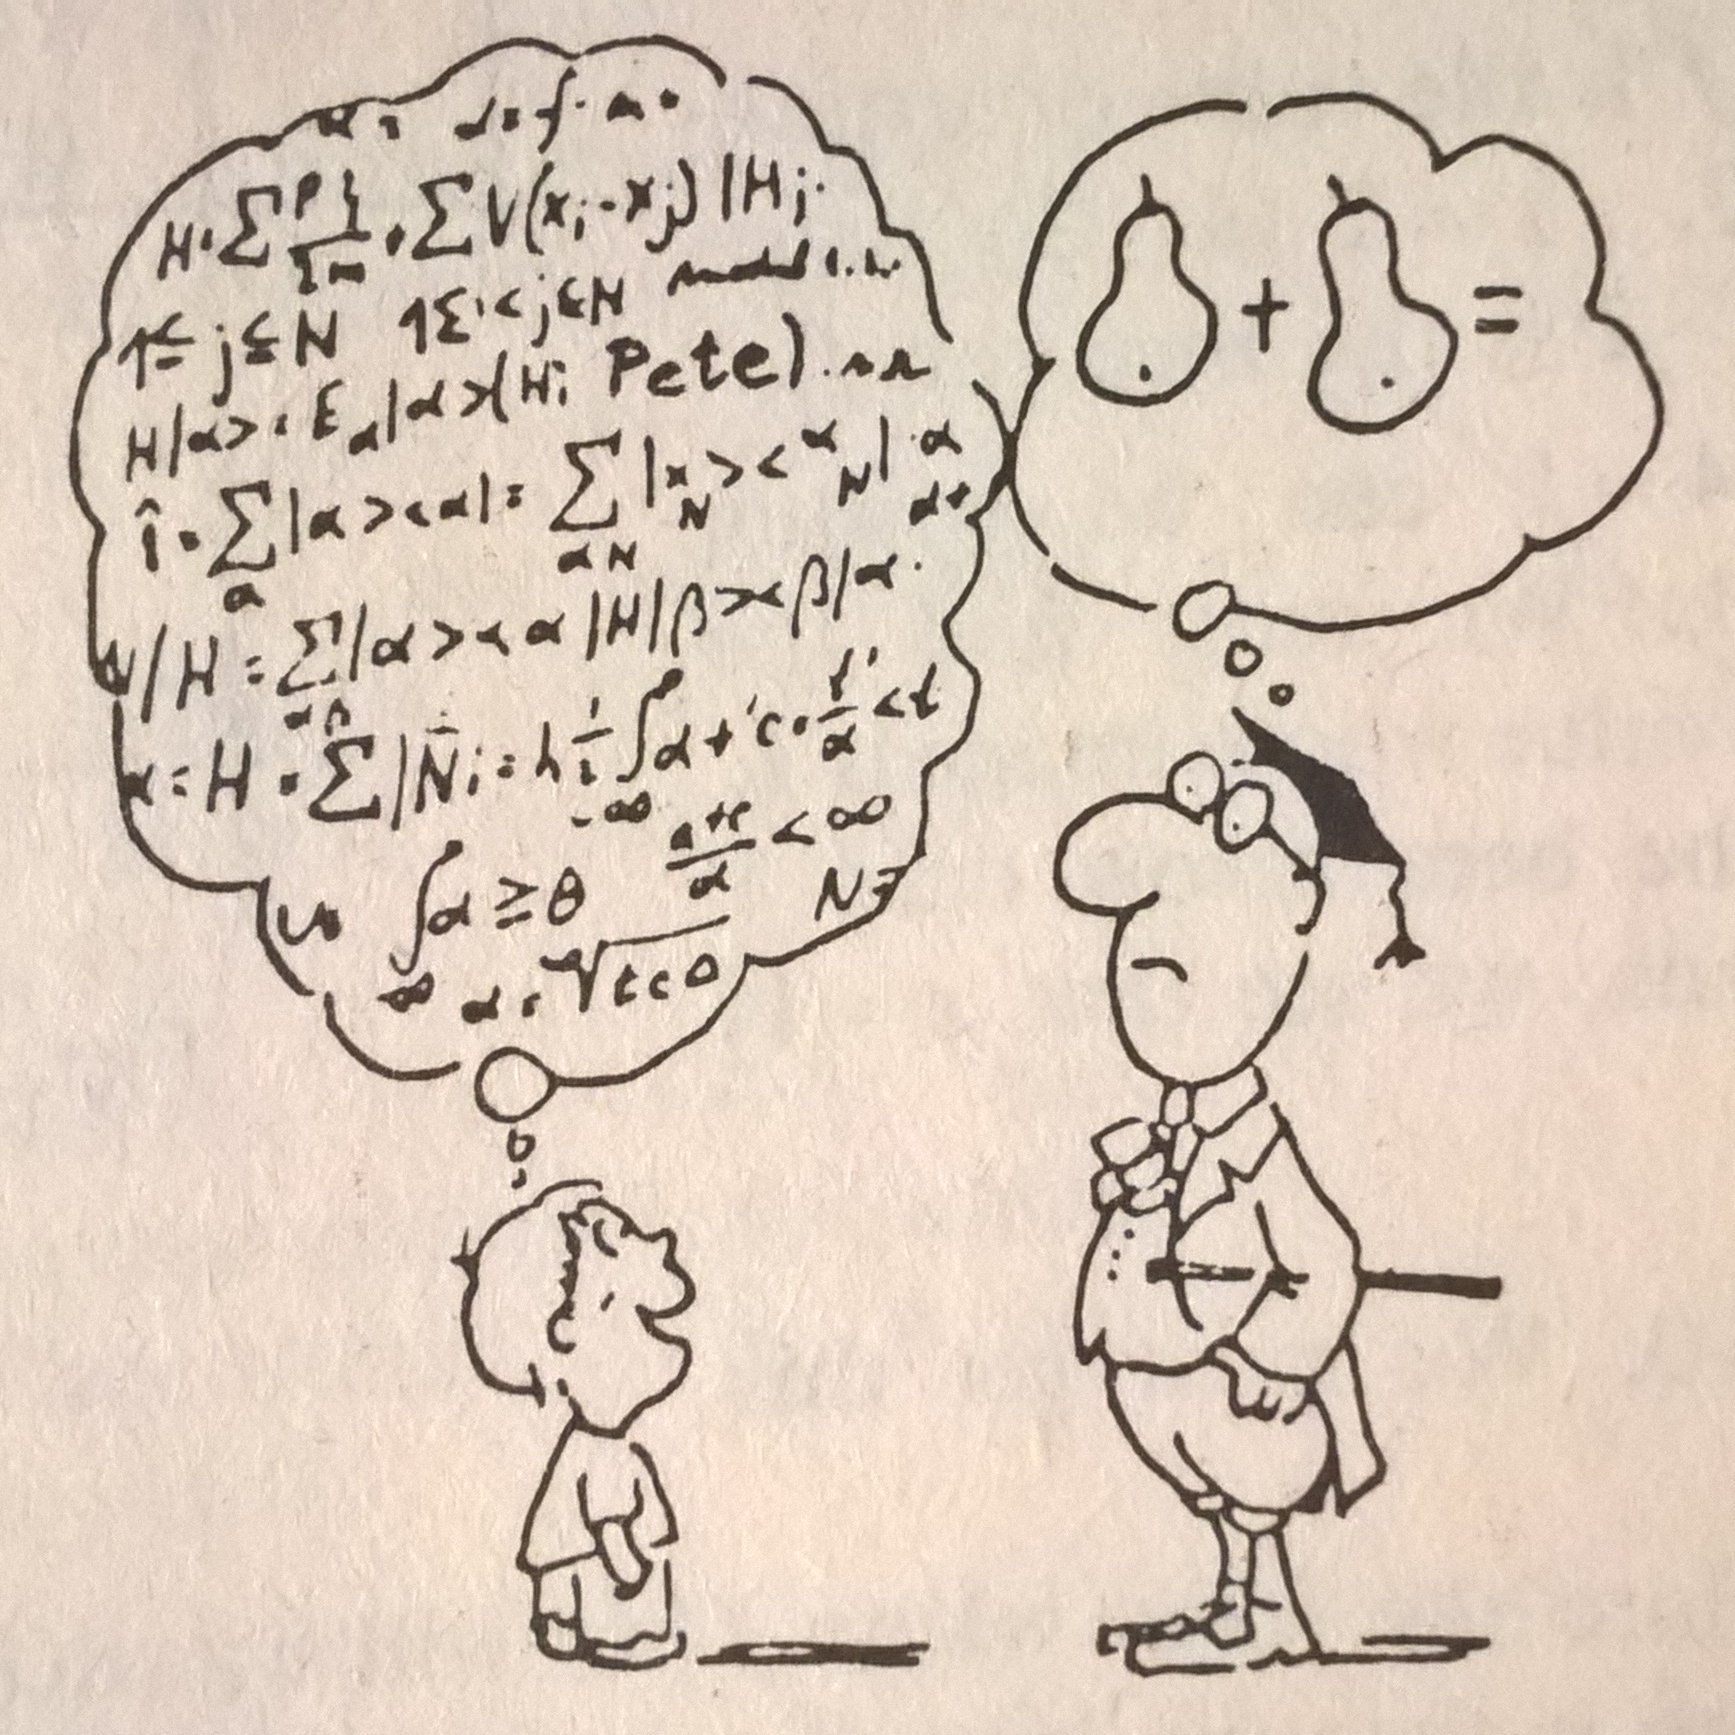
\includegraphics[scale=0.25]{./image/Math/doubts.jpg}
\end{minipage}

\newpage
\section{Definition}
\Large
\subsection{Exponents}
\begin{enumerate}
\item 
\[a^n \; = \; a \times a \times a \times a \; .... \; n \quad factors \qquad (n \in \mathbb{N}, \; a \in \mathbb{R})\]
\item 
\[a^{-m} \; = \; \frac{1}{a^m} \qquad (m \in \mathbb{Z^+}, \; a \in \mathbb{R}, \; a \neq 0)\] \\
and \\
\[\frac{1}{a^{-m}} \; = \; a^m\]
\item 
\[a^0=1 \qquad (a \in \mathbb{R}, \; a \neq 0)\]
\end{enumerate}
\subsection{Rational Exponents:}
\begin{enumerate}
\item
\[\sqrt[n]{a} \; = \; r \qquad (a \; > \; 0, \; n \in \mathbb{N}, \; n \geqslant 2, \; r \; > \; 0), \; \Longleftrightarrow \; r^n \; = \; a\]
\item
\[a^{\frac{1}{n}} \; = \; \sqrt[n]{a}; \qquad (a \; > \; 0, \; n \; \geqslant 2, \; n \in \mathbb{N})\]
\item
\[a^{\frac{-1}{n}} \; = \; \sqrt[n]{a^{-1}}; \qquad (a \; > \; 0, \; n \; > 0, \; n \in \mathbb{N} )\]
\item
\[a^{\frac{m}{n}} \; = \; \sqrt[n]{a^m}; \qquad (a \; > \; 0; \; m, \; n \in \mathbb{Z}, \; n \geqslant 2 )\]
\end{enumerate}
\newpage
\section{Law}
\subsection{Exponents}
\begin{enumerate}
\item
\[a^m \; \times \; a^n \; = a^{m+n} \qquad (m, \; n \in \mathbb{N})\]
\[a^m \; \times \; a^n \; = a^{m+n} \qquad (m, \; n \in \mathbb{Z}; \; a \neq 0, \; if \quad m \quad or \quad n \; < \; 0)\]
\item
\[\frac{a^m}{a^n}=a^{m-n} \qquad (m, \; n \in \mathbb{Z}; \; a \in \mathbb{R}; \; a \neq 0)\]
\item
\[(ab)^m \; = \; a^m \; b^m \qquad (m \in \mathbb{Z})\]
\item
\[(a^m)^n \; = \; a^{mn} \qquad (m, \; n \in \mathbb{Z})\]
\end{enumerate}
\subsection{Rational Exponents}
\begin{enumerate}
\item
\[a^r \; \times \; a^t \; = \; a^{r+t} \qquad (a \; > \; 0; \quad r, \; t \in \mathbb{Q})\]
\item
\[\frac{a^r}{a^t}=a^{r-t} \qquad (a \; > \; 0; \quad r, \;t \in \mathbb{Q})\]
\item
\[(a^t)^r \; = \; a^{tr} \qquad (a \; > \; 0, \quad t, \; r \in \mathbb{Q})\]
\item
\[(ab)^t \; = \; a^t \; b^t \; ; \quad \left(\frac{a}{b}\right)^t \; = \; \frac{a^t}{b^t} \; ; \qquad (a, \; b \; > \; 0, \quad t \in \mathbb{Q})\]
and\\
\[a^t \; b^t \; = \; (ab)^t \qquad and \qquad \frac{a^t}{b^t} \; = \; \left(\frac{a}{b}\right)^t\]
\end{enumerate}
\subsection{Distributive law}
\[a(b \; + \; c) \; = \; ab \; + \; ac\]
\begin{align*}
(a \; + \; b)(c \; + \; d) \; &= \; (a \; + \; b)c \; + \; (a \; + \; b)d \\
&=ac \; + \;bc \; + \; ad \; + \; bd
\end{align*}
\[A^2 \; - \; B^2 \; = \; (A \; - \; B)(A \; + \; B)\]
\subsection{Commutative law}
\[ab \; = \; ba\]
\section{Properties}
\subsection{Addition}
\[0 \; + \; a \; = \; a\]
\[\frac{a}{b} \; + \; \frac{c}{b} \; = \; \frac{a \; + \; c}{b} \qquad (b \; \neq \; 0)\]
\[\frac{a}{b} \; - \; \frac{c}{b} \; = \; \frac{a \; - \; c}{b} \qquad (b \; \neq \; 0)\]
\subsection{Multiplication}
\[0 \times a \; = \; 0\]
\[\frac{0}{a} \; = \; 0 \times \frac{1}{a} \; = \; 0\]
\[1 \times a \; = \; a\]
\[\frac{a}{b} \times \frac{c}{d} \; = \; \frac{ac}{bd} \qquad (b \; \neq \; 0; \; d \; \neq \; 0)\]
\subsection{Division}
\[\frac{a}{0} \; = \; undefined\]
\[\frac{p}{q} \div \frac{r}{s} \; = \; \frac{p}{q} \times \frac{s}{r} \; = \; \frac{ps}{qr} \qquad (q \; \neq \; 0; \; r \; \neq \; 0; \; s \; \neq \; 0)\]
\\
\\
\begin{minipage}{\linewidth}
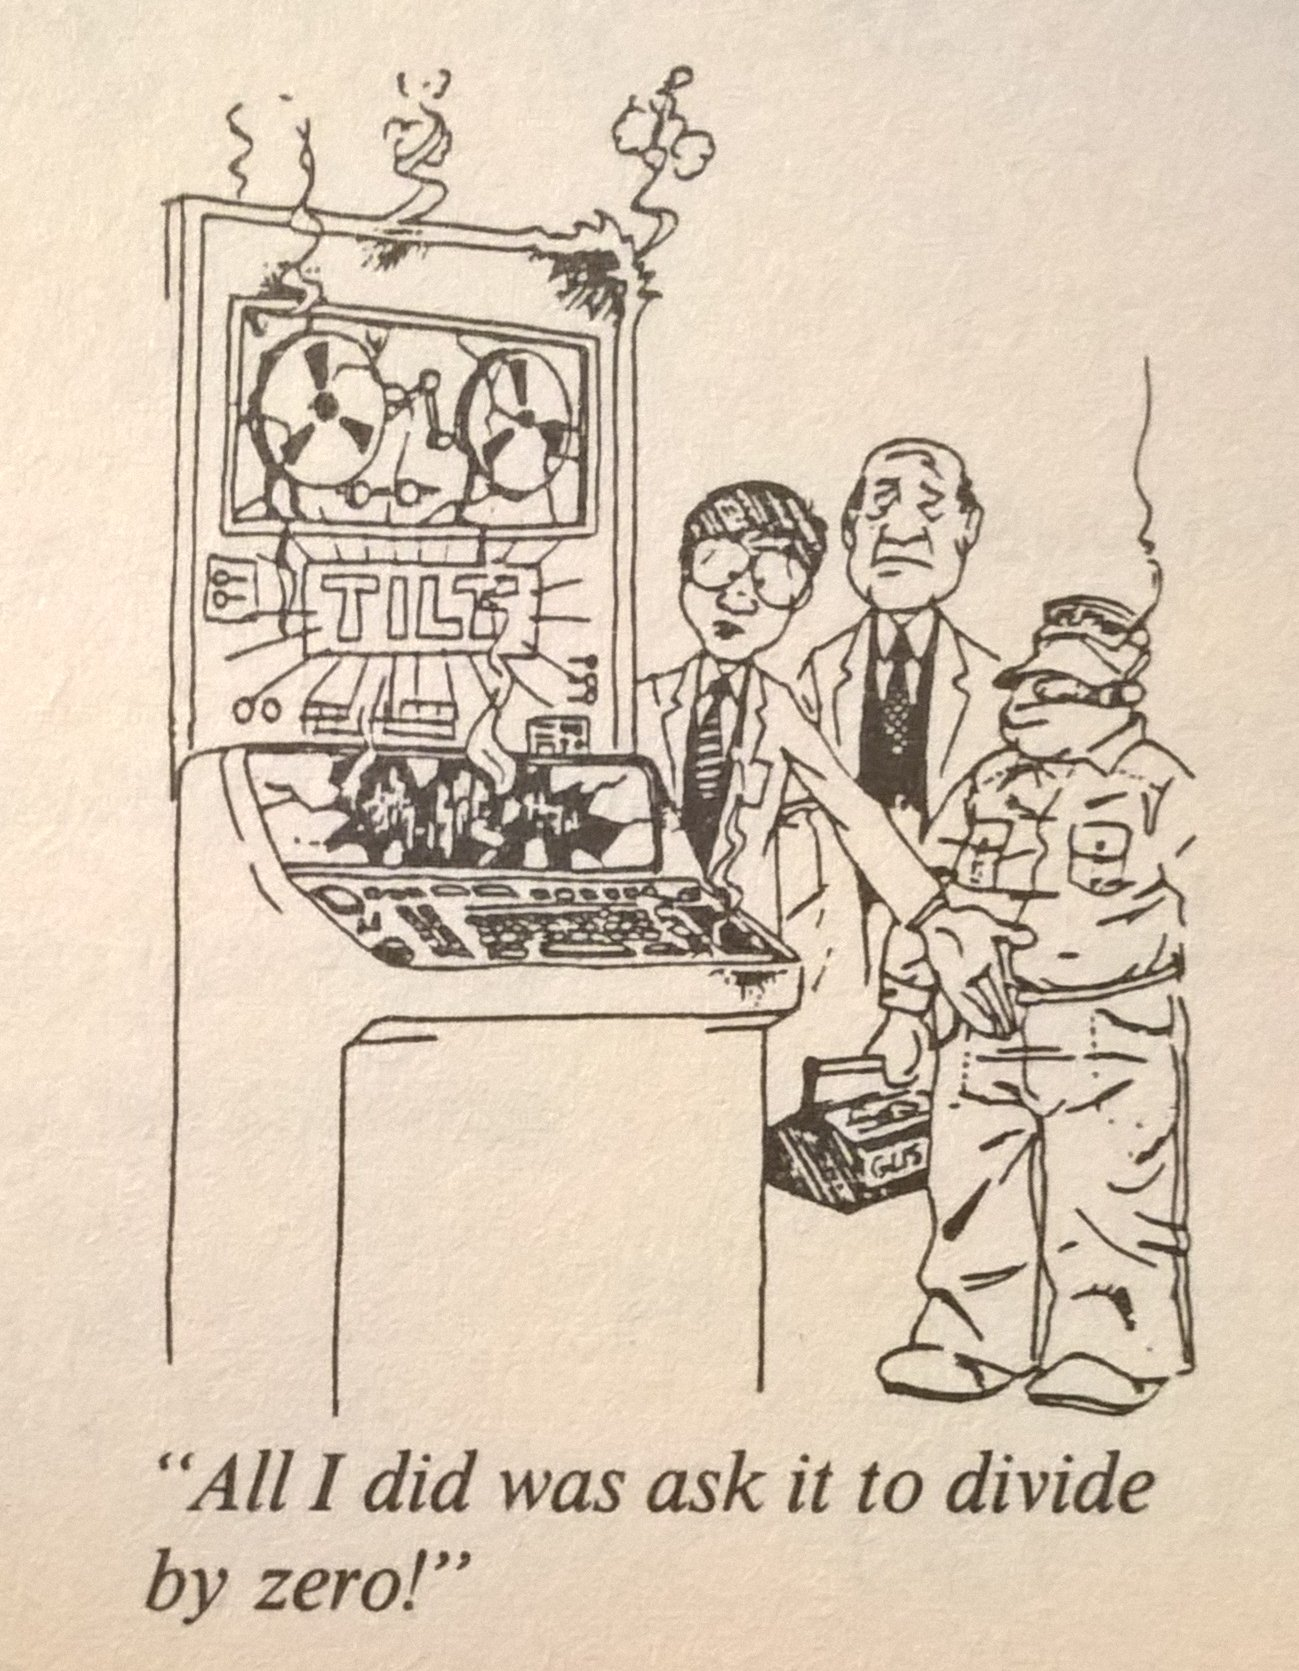
\includegraphics[scale=0.2]{./image/Math/dividebyzero.jpg}
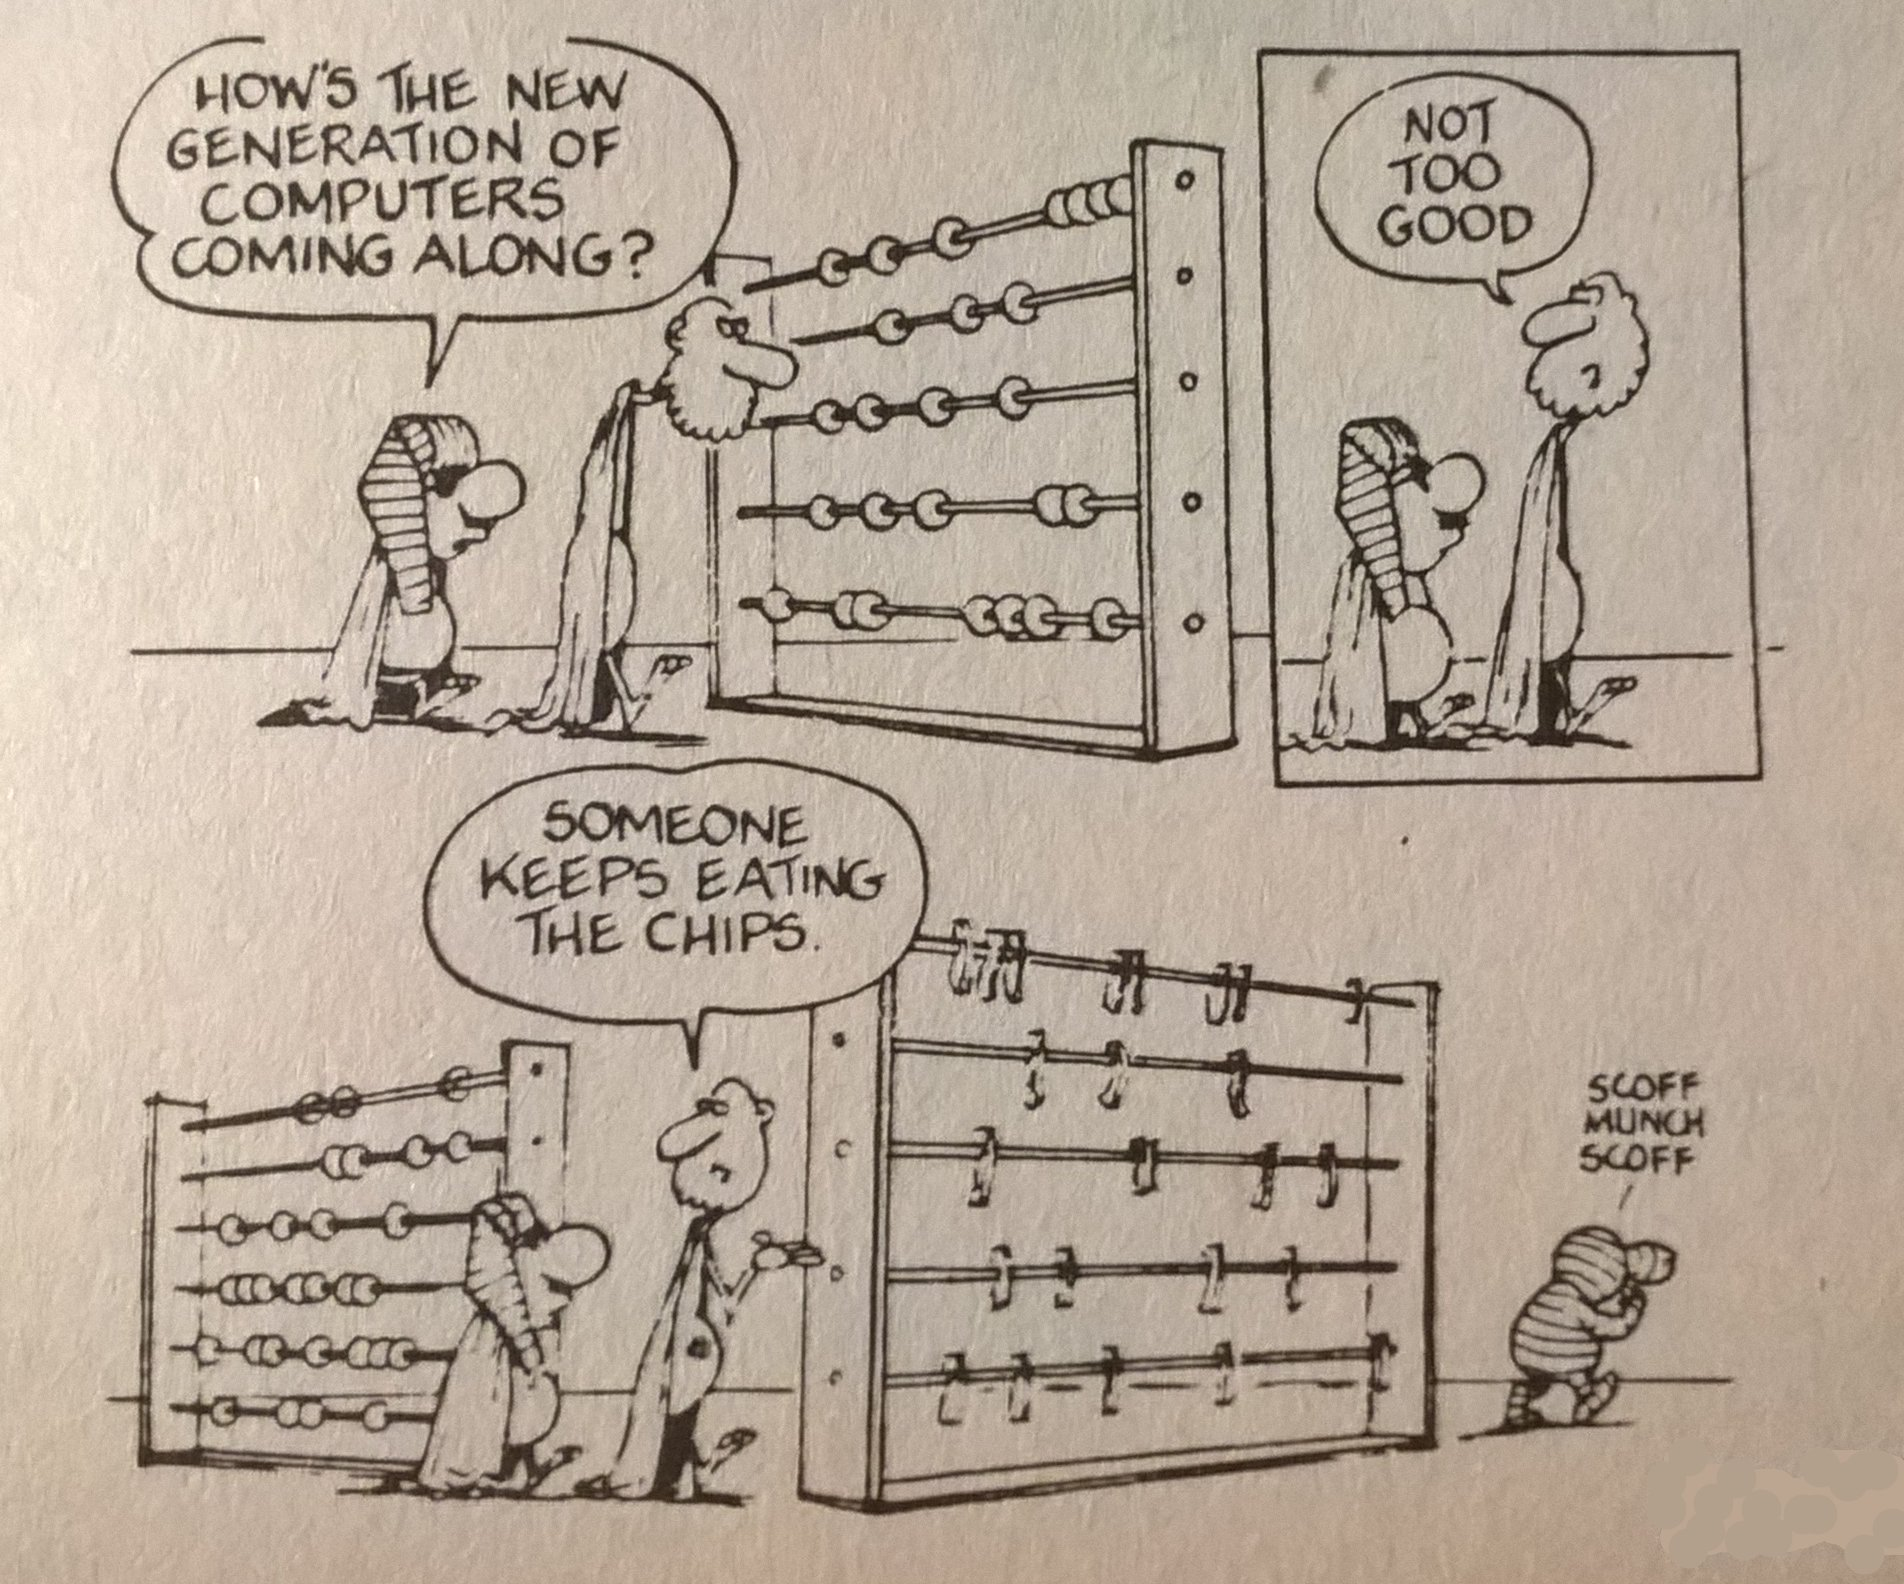
\includegraphics[scale=0.12]{./image/Math/newgencomputer.jpg}
\end{minipage}
\\
\\
\section{Examples}
\begin{minipage}{\linewidth}
	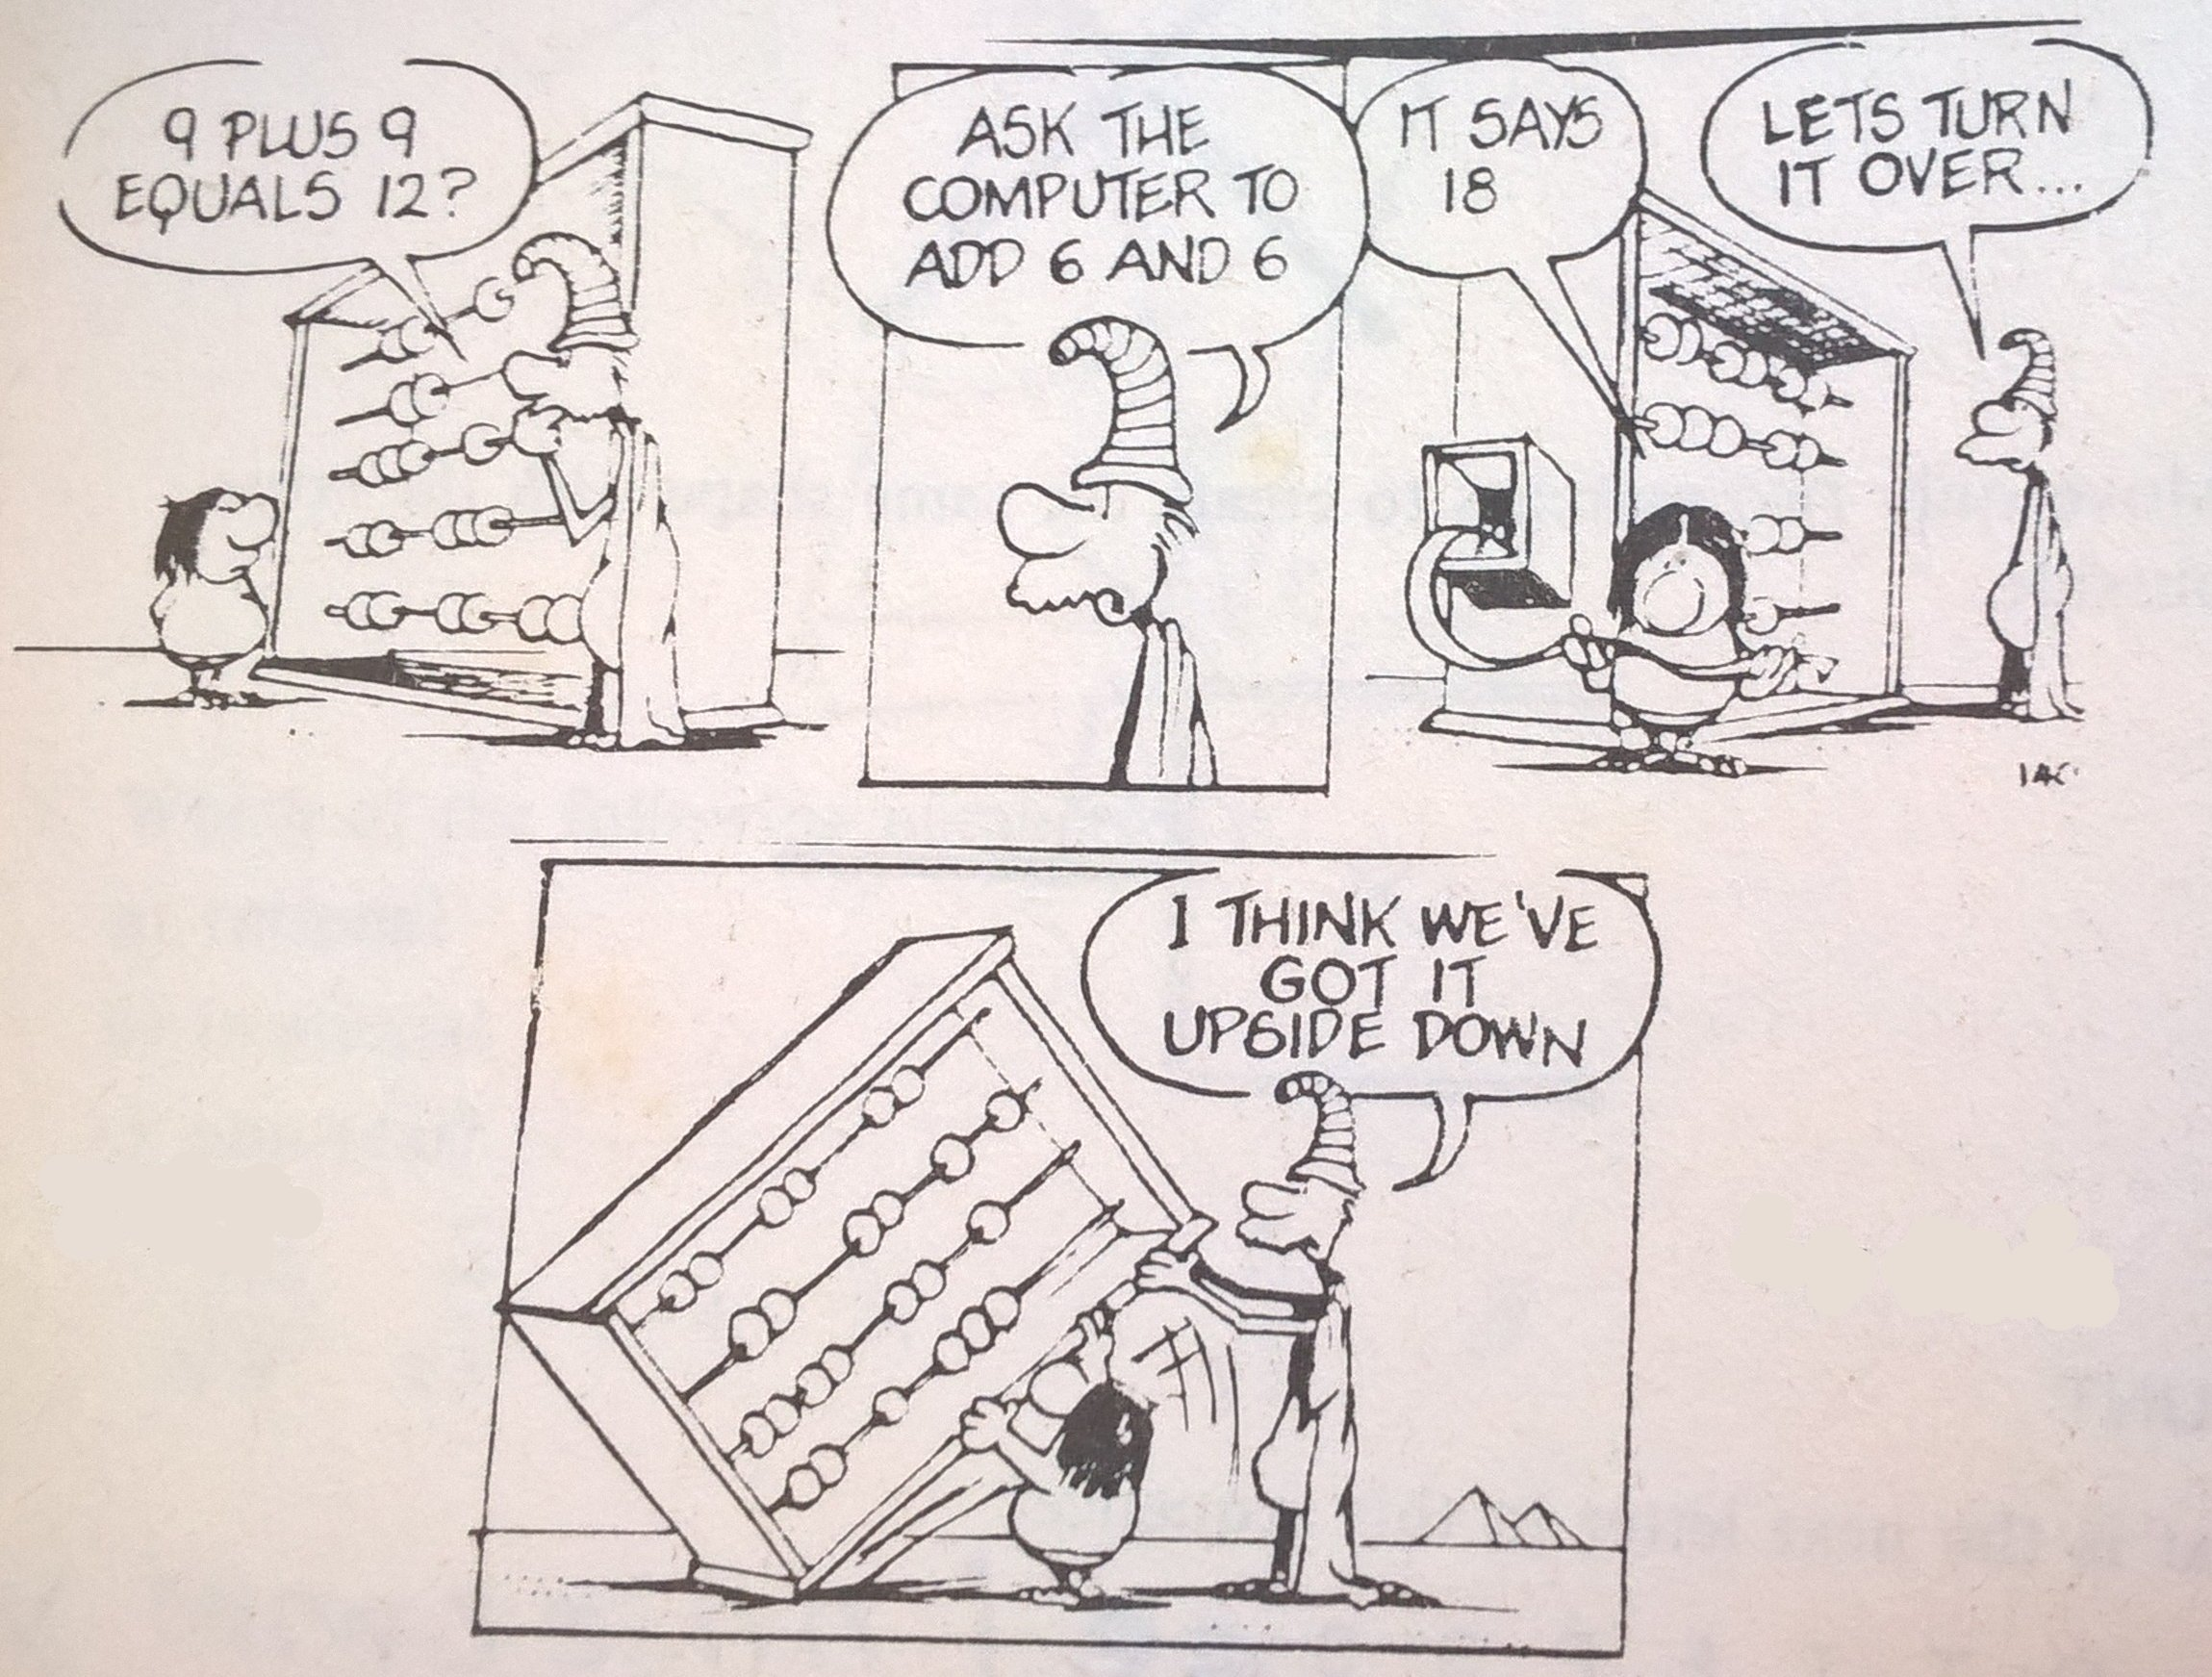
\includegraphics[scale=0.2]{./image/Math/upsidedown.jpg}
\end{minipage}
\subsection{}
\[\sqrt{a^2} \; = \; a \qquad (a \; > \; 0) \qquad \qquad \sqrt{a^n} \; = \; a^{\frac{n}{2}}\] \\
\[\sqrt{\frac{1}{a}} \; = \; \frac{1}{\sqrt{a}}\] \\
\[a^{\frac{m}{1}} \; = \; a^m \qquad \qquad \frac{a^m}{a^n} \; = \; a^{m-n}\] \\
\[\frac{a \; \angle \alpha^\circ \; b \; \angle \beta^\circ}{c \; \angle \gamma^\circ} \; = \; \frac{a \times b}{c} \quad \angle \; (\alpha^\circ + \beta^\circ - \gamma^\circ)\]
\\
\[If \quad a \; . \; b \; = \; 0, \quad then \quad a \; = \; 0 \quad or \quad b \; = \; 0\]
\\
\\








\section{Methods}
HCF - highest common factor (pôr variável em evidência) \\
CF - Common factors \\
Factorisation \\
LCD or LCM - Lowest common denominator or lowest common multiple \\
%%%%%%%%%%%%%%%%%%%%%%%%%%%%%%%%%%%%%%%%%%%%%%%%%%%%%%%%%%%%%%%%%%%%%%%%%%%%%%%%
\newpage
\normalsize
\null \vfill
%\vspace*{\fill}
\textit{Eng. Sérgio Santos}
\end{document}
%%%%%%%%%%%%%%%%%%%%%%%%%%%%%%%%%%%%%%%%%%%%%%%%%%%%%%%%%%%%%%%%%%%%%%%%%
\begin{comment}
hello
\huge
$\mcirc \msquare   \triangle \bigtriangleup \triangleleft \bigcirc \square  \Box \Diamond$
\normalsize
pôr em evidência (factorisation)\\
dominador comum\\
frações parciais\\
\vspace{10cm}
$\frac{\square}{\square}=1$
HCF - highest common factor \\
Factorization \\
LCD or LCM - Lowest common denominator or lowest common multiple \\
\end{comment}
%%%%%%%%%%%%%%%%%%%%%%%%%%%%%%%%%%%%%%%%%%%%%%%%%%%%%%%%%%%%%%%%%